\documentclass[conference]{IEEEtran}

\usepackage{graphicx}
\usepackage{amsmath}
\usepackage{kotex}
\usepackage{url}

\title{권장과목 기반 학과 군집화: 입시 상담 지원을 위한 탐색적 분석}

\author{
  \IEEEauthorblockN{박재우}
  \IEEEauthorblockA{NOVA50301 Term Project --- Progress Report}
}

\begin{document}
\maketitle

\begin{abstract}
본 연구는 고등학교 권장과목 정보가 대학 학과들을 해석 가능한 방식으로 군집화할 수 있는지를 탐색한다.
울산 지역 산업 맥락을 반영한 25개 학과(조선해양ㆍ자동차공학 포함)를 대상으로 cosine similarity 기반 hierarchical clustering과 k-means를 적용하였다.
$k=4$에서 STEM-보건 대군집, 사회/상경 군집, 국어국문 singleton, 디자인 singleton의 안정적 구조가 확인되었으며, 외부 검증을 위한 현직 입시교사 14명 대상 card sorting을 병행 진행 중이다.
\end{abstract}

\section{Introduction \& Data}

본 프로젝트는 완성된 학과 추천 시스템이 아니라 권장과목 profile을 통한 학과 간 준비과목 유사성을 분석하는 탐색적 군집화 연구이다.
분석 대상은 25개 학과(인문/사회/상경 7, 자연/공학/의약 18)로, 통계적 대표 표본이 아니라 (i) 권장과목 다양성, (ii) 입시 상담 출현 빈도, (iii) 해석 가능성을 고려한 목적 표본이다.
특히 조선해양공학과ㆍ자동차공학과는 울산 지역 주력 산업 맥락을 반영한 industry-specific engineering boundary case로 포함하였다.
원자료는 학과 과목 선택 가이드이며, 각 학과-과목 값은 권장과목으로 제시되면 1, 미언급이면 0으로 코딩하였다(25 $\times$ 92 binary matrix).

\section{Methods}

학과 vector 간 유사도는 cosine similarity를 사용하였다.
이는 학과별 권장과목 수 차이를 normalization하고, sparse vector에서 구성 패턴 비교를 우선하기 위함이다.
군집화는 두 방법을 비교하였다:
(i) Hierarchical clustering(average linkage) --- 소표본에서 dendrogram 해석이 용이하고 사전 $k$가 불필요하다;
(ii) K-means clustering($k=2$--$8$) --- silhouette score(cosine), Davies-Bouldin(DB) index로 정량 평가하였다.

\section{Preliminary Results}

\subsection{군집 구조}

Cosine distance $\approx 0.78$에서 명확한 컷이 형성되어 $k=4$ anchor 구조가 나타난다:
(a) STEM-보건-공학 17개 학과 대군집(자동차공학ㆍ조선해양공학ㆍ의예ㆍ약학 등 포함),
(b) 사회과학ㆍ상경 6개 학과(심리ㆍ경영ㆍ사회ㆍ경제ㆍ미디어커뮤니케이션ㆍ사학),
(c) 국어국문학과 singleton,
(d) 디자인학과 singleton.

울산 산업 boundary case의 위치가 명확히 드러난다.
자동차공학과는 기계공학과($\cos=0.951$), 전기전자공학과($\cos=0.901$), 컴퓨터공학과($\cos=0.781$)와 매우 높은 유사도를 보여 modern engineering hub의 중심에 위치한다.
조선해양공학과는 신소재ㆍ화학ㆍ화학공학과와 묶이는 material-chemistry engineering subcluster에 속한다.

\begin{figure}[t]
  \centering
  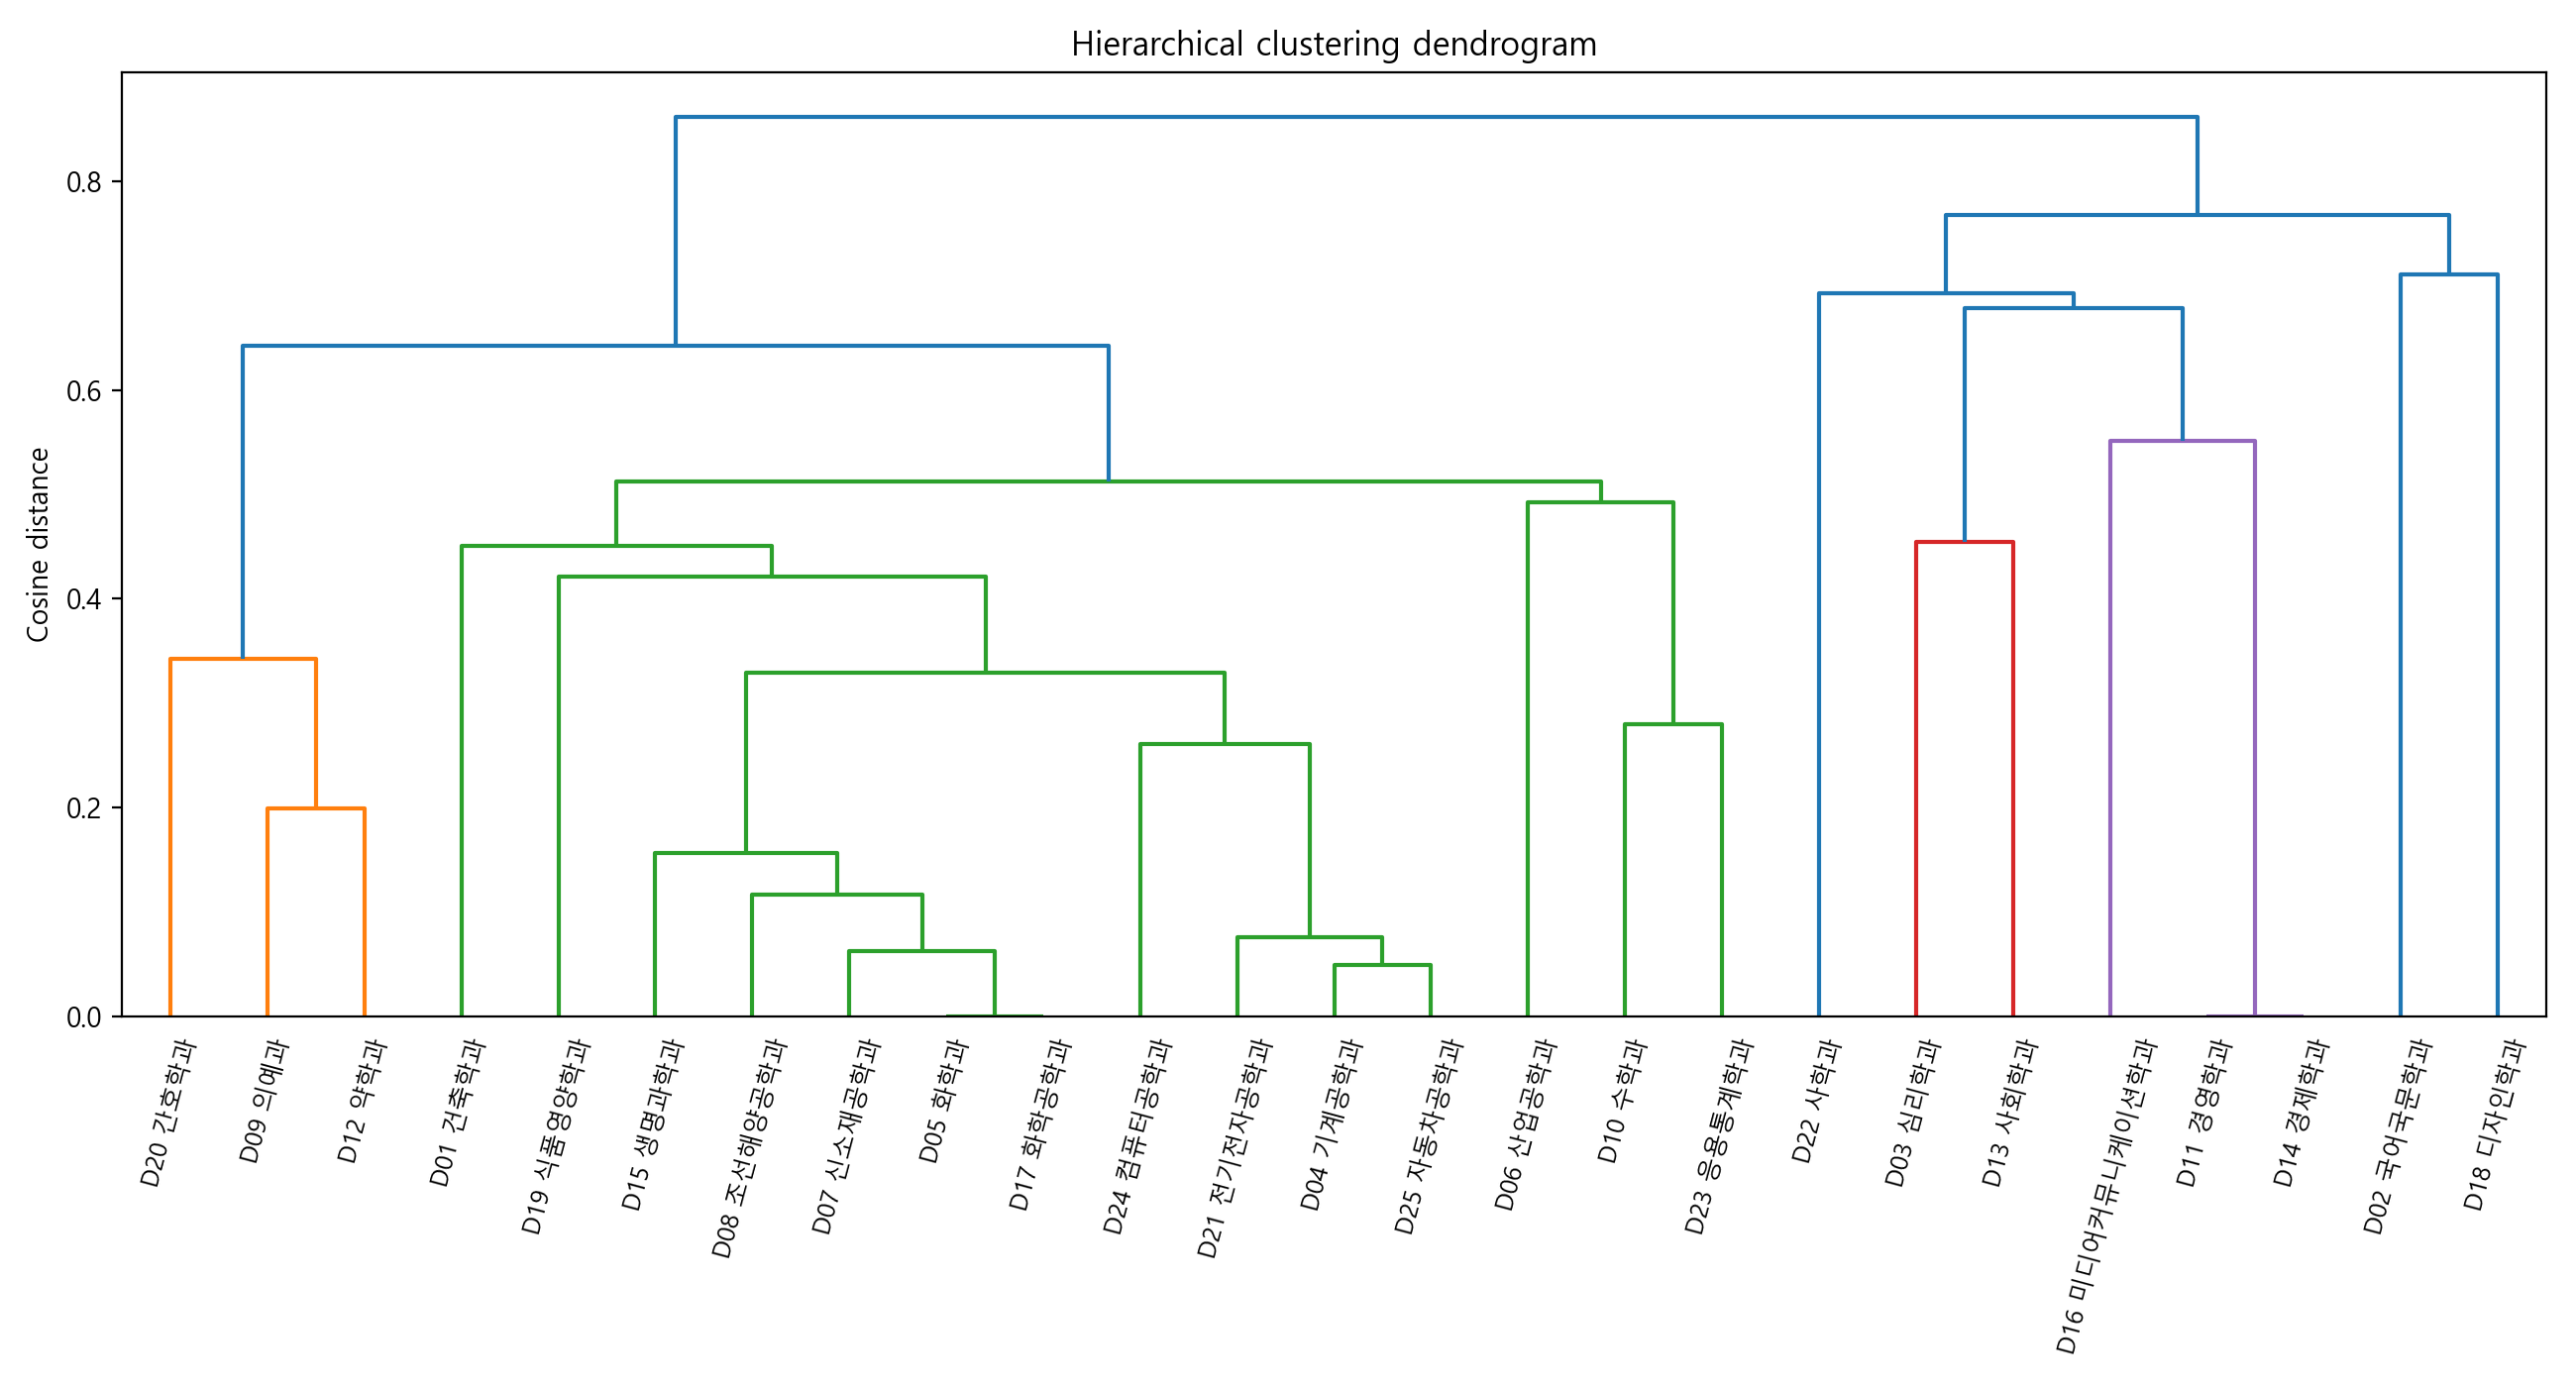
\includegraphics[width=\linewidth]{hierarchical_dendrogram.png}
  \caption{Dendrogram(average linkage, cosine distance). 자동차공학과는 기계공학과와 가장 작은 거리에서 결합하며, 국어국문학과ㆍ디자인학과의 isolation이 시각적으로 확인된다.}
  \label{fig:dendrogram}
\end{figure}

\subsection{정량 평가 \& 학과 쌍 발견}

Silhouette은 $k=6$에서 최고(0.347), DB는 $k=8$에서 최저(1.154)였다.
$k=4$(anchor)에서 silhouette은 0.290, DB는 1.442로 절대값은 최고가 아니지만 해석 가능성-세분성 trade-off에서 가장 균형적이다.
$k$가 커질수록 사회과학 군집이 (심리-사회)와 (경영-경제-미디어)로 분화되나, 단일 학과 singleton이 늘어 해석이 산만해진다.

학과 쌍 단위로는 화학과-화학공학과 $\cos=1.000$(권장과목 완전 동일), 경영학과-경제학과 $\cos=1.000$, 기계공학과-자동차공학과 $\cos=0.951$, 기계공학과-전기전자공학과 $\cos=0.947$ 등 직관과 일치하는 고유사도 페어가 관찰되었다.
사학과는 어떤 STEM 학과와도 유사도가 0에 가까워 인문/STEM 경계가 매우 명확함을 보여준다.

\section{Expert Validation --- Card Sorting}

내부 평가 지표는 군집의 기하학적 특성만 측정하므로, 본 연구는 외부 기준으로 현직 입시교사 14명의 card sorting 결과를 활용한다.
Task는 open card sort이며, 25개 학과 카드를 ``권장과목 관점에서 비슷한 학과끼리'' 그룹 수 제한 없이 자유롭게 분류한다(평가자의 독립적 직관을 최대한 보존하기 위해 사전 $k$를 강제하지 않는다).
Analysis 단계에서는 14명 분류를 $25 \times 25$ co-occurrence(동시분류 빈도) matrix로 집계하여 consensus clustering을 도출하고, 이를 $k=4$ㆍ$k=6$ 수준에서 잘라 hierarchical/k-means 결과와 Adjusted Rand Index(ARI), Normalized Mutual Information(NMI), pairwise agreement로 비교한다.
현재 템플릿 설계는 완료되었으며 W14에 응답 수집, Final Report에서 정량 일치도를 보고한다.

\section{Limitations \& Next Steps}

본 연구의 한계는 다음과 같다.
첫째, 25개 학과는 목적 표본이므로 일반화에 한계가 있다.
둘째, STEM-보건 17개가 한 군집에 묶이는 현상은 권장과목 해상도의 한계, 즉 수학ㆍ과학 과목명만으로 세부 전공 차이를 충분히 반영하지 못할 가능성을 시사한다.
셋째, card sorting 응답은 아직 수집 전이다.

Final report에서는 (a) card sorting 기반 ARI/NMI 일치도 분석, (b) STEM 대군집 내부 sub-clustering, 특히 modern engineering vs. material-chemistry vs. medical-health 세분화, (c) hierarchical과 k-means 할당 일치도 비교를 진행한다.

\end{document}
